\documentclass{article}\usepackage[]{graphicx}\usepackage[]{color}
%% maxwidth is the original width if it is less than linewidth
%% otherwise use linewidth (to make sure the graphics do not exceed the margin)
\makeatletter
\def\maxwidth{ %
  \ifdim\Gin@nat@width>\linewidth
    \linewidth
  \else
    \Gin@nat@width
  \fi
}
\makeatother

\definecolor{fgcolor}{rgb}{0.345, 0.345, 0.345}
\newcommand{\hlnum}[1]{\textcolor[rgb]{0.686,0.059,0.569}{#1}}%
\newcommand{\hlstr}[1]{\textcolor[rgb]{0.192,0.494,0.8}{#1}}%
\newcommand{\hlcom}[1]{\textcolor[rgb]{0.678,0.584,0.686}{\textit{#1}}}%
\newcommand{\hlopt}[1]{\textcolor[rgb]{0,0,0}{#1}}%
\newcommand{\hlstd}[1]{\textcolor[rgb]{0.345,0.345,0.345}{#1}}%
\newcommand{\hlkwa}[1]{\textcolor[rgb]{0.161,0.373,0.58}{\textbf{#1}}}%
\newcommand{\hlkwb}[1]{\textcolor[rgb]{0.69,0.353,0.396}{#1}}%
\newcommand{\hlkwc}[1]{\textcolor[rgb]{0.333,0.667,0.333}{#1}}%
\newcommand{\hlkwd}[1]{\textcolor[rgb]{0.737,0.353,0.396}{\textbf{#1}}}%
\let\hlipl\hlkwb

\usepackage{framed}
\makeatletter
\newenvironment{kframe}{%
 \def\at@end@of@kframe{}%
 \ifinner\ifhmode%
  \def\at@end@of@kframe{\end{minipage}}%
  \begin{minipage}{\columnwidth}%
 \fi\fi%
 \def\FrameCommand##1{\hskip\@totalleftmargin \hskip-\fboxsep
 \colorbox{shadecolor}{##1}\hskip-\fboxsep
     % There is no \\@totalrightmargin, so:
     \hskip-\linewidth \hskip-\@totalleftmargin \hskip\columnwidth}%
 \MakeFramed {\advance\hsize-\width
   \@totalleftmargin\z@ \linewidth\hsize
   \@setminipage}}%
 {\par\unskip\endMakeFramed%
 \at@end@of@kframe}
\makeatother

\definecolor{shadecolor}{rgb}{.97, .97, .97}
\definecolor{messagecolor}{rgb}{0, 0, 0}
\definecolor{warningcolor}{rgb}{1, 0, 1}
\definecolor{errorcolor}{rgb}{1, 0, 0}
\newenvironment{knitrout}{}{} % an empty environment to be redefined in TeX

\let\hlesc\hlstd \let\hlpps\hlstd \let\hllin\hlstd \let\hlslc\hlcom \let\hlppc\hlcom
\usepackage{alltt}
\usepackage{natbib}
\usepackage[unicode=true]{hyperref}
\usepackage{geometry}
\usepackage{hyperref}
\usepackage{color}
\usepackage{amsmath}
\usepackage{amssymb}
\usepackage{verbatim}
\usepackage{mathpazo}
\usepackage{setspace}
\usepackage{multirow}
\usepackage{fullpage}
\usepackage{lscape}
\usepackage{fancyhdr}
\usepackage{wrapfig,lipsum,booktabs}
\usepackage[normalem]{ulem}
\usepackage[parfill]{parskip}
\usepackage{multirow}
\geometry{tmargin=1in,bmargin=1in,lmargin=1in,rmargin=1in}

\bibliographystyle{ecology_let}

%% for inline R code: if the inline code is not correctly parsed, you will see a message
\newcommand{\rinline}[1]{SOMETHING WRONG WITH knitr}


\IfFileExists{upquote.sty}{\usepackage{upquote}}{}
\begin{document}
\title{Opportunistic attachment assembles plant-pollinator networks: A walk through of the analysis}
\author{Lauren Ponisio}

\maketitle

\begin{figure}[h!]
  \centering
  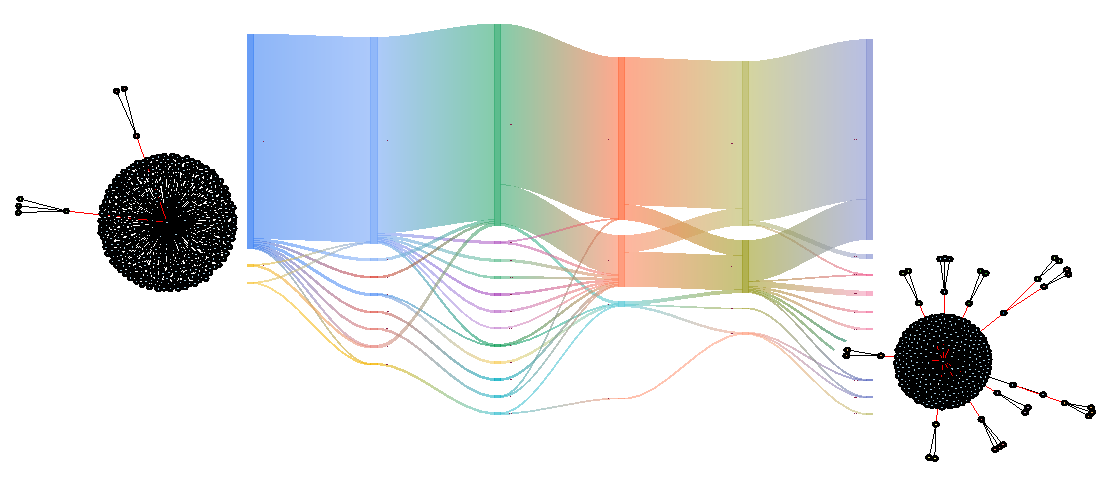
\includegraphics[width=1.1\textwidth]{figure/SankeyIDb303b2e99ce.pdf}
  \label{fig:methods}
\end{figure}
\clearpage

\section{Overview}
\label{sec:overview}

In our study we examin the temporal dynamics of plant-pollinator
network assembly using variety of different methods including 1) network
change point detection 2) node/species-level position variation, 3)
species and interaction turnover 4) network-level metrics and 5)
extinction simulations. We are committed to reproducible science and
all analytical code will be maintained on github, along with this
write up.

The entire analysis is executable from the main.sh file. All of the
packages needed to run the analyses are listed in the packages.sh
file, including the specific versions of the python dendropy library,
which is very finicky. We have had no problems with backward
compatibility for the R scripts (in terms of R versions from v.~2-3.4
or packages) but the change point analysis must be run in python2 (not
easily convertible to python3, though this is potentially in
progress).

Navigate to the analysis folder within the github repo
(hedgerow\_assembly) then the main.sh file can be selected and
run. I would not recommend doing this unless you are prepared to have two
cores of your machine running for days to weeks (depending on how many
of iterations of the change point analysis specific in
mainChangePoint.sh loop), but you could run of the analyses in the
study by running this line in BASH.

\begin{knitrout}
\definecolor{shadecolor}{rgb}{0.969, 0.969, 0.969}\color{fgcolor}\begin{kframe}
\noindent
\ttfamily
\hlstd{\ bash\ main.sh}\hspace*{\fill}
\mbox{}
\normalfont
\end{kframe}
\end{knitrout}

This will somewhat helpfully print the results of each analysis
and re-create any accompanying figures.

We will walk through each the main script for each analysis
individually.


\section{Change Point Analysis}

The change point analysis which is a mix of python and R. hedgerows.py
(the meat of the change point analysis) runs in parallel on two cores
(which can be modified in the hedgerows.py script by toggling the
ncores object), but will likely take a many hours (a day on running on
my 2.5 GHz Intel Core i7 mac pro) depending on your machine.

There is some stochasticity in the change point analysis in the
hypothesis testing step where samples are drawn from the null
distribution and the likelihood of a change point occurring is
calculated from those samples. Because of this, we re-ran the change
point detection analysis 1000 times (this was done on a cluster) and
used the change points that were identified in 95\% of runs in
subsequent analyses.

mainChangePoint.sh compiles the python code, then creates the .pairs
files needed for the change point analysis (dataPrep.R). Nodes names
need to be consistent across years within a site, and for simplicity
we made them consistent across all sites as well. This enabled us to
provide a single .lut master list of the nodes to the analysis.

Next, the change point detection loop is run. This function begins by
fitting the generalized hierarchical random graph model (GHRG) which
outputs consensus trees that are used by the change point detection
algorithm. There is only slight variability in the fitting of the
GHRG between runs, so once the first loop is run, the consensus trees
are used in subsequent runs.

The output of the change point analysis is saved as a list of the
change points identified and likelihood scores (formatted by
prepChangePointOutput.R).

After the loop, consensusChangePoints.R drops the change points that
were not identified by $95\%$ of the runs and then creates consensus
trees for each chunk of years between change point in python
(postChangePoint.py). The outputs of the change point analysis were
very specialized to that analysis, so we had to convert them to .glm
files for plotting and further exploration in R
(convertConsensusTrees.py)

The plotting and statistical analyses are in R in different
scripts. The plotting function will create the network, community and
flow plots (networks.R). The binomial linear mixed models are run in
the comparison.R script, along with addition statistical analysis
requested by the reviewers testing whether change points tended to
occur between years with a larger difference in samples.




\begin{knitrout}
\definecolor{shadecolor}{rgb}{0.969, 0.969, 0.969}\color{fgcolor}\begin{kframe}
\begin{alltt}
\hlstd{mod.chpt} \hlkwb{<-} \hlkwd{glm}\hlstd{(}\hlkwd{cbind}\hlstd{(chpt.trial}\hlopt{$}\hlstd{chpts,}
                      \hlstd{chpt.trial}\hlopt{$}\hlstd{trial} \hlopt{-} \hlstd{chpt.trial}\hlopt{$}\hlstd{chpts)} \hlopt{~}
    \hlstd{chpt.trial}\hlopt{$}\hlstd{status,} \hlkwc{family}\hlstd{=}\hlstr{"binomial"}\hlstd{)}
\hlkwd{print}\hlstd{(}\hlkwd{summary}\hlstd{(mod.chpt))}
\end{alltt}
\begin{verbatim}
## 
## Call:
## glm(formula = cbind(chpt.trial$chpts, chpt.trial$trial - chpt.trial$chpts) ~ 
##     chpt.trial$status, family = "binomial")
## 
## Deviance Residuals: 
##      Min        1Q    Median        3Q       Max  
## -1.67612  -0.46233  -0.42803  -0.09731   1.67955  
## 
## Coefficients:
##                          Estimate Std. Error z value Pr(>|z|)    
## (Intercept)               -1.5041     0.4513  -3.333 0.000861 ***
## chpt.trial$statusmature   -0.8473     0.8668  -0.978 0.328315    
## chpt.trial$statuscontrol  -2.6703     1.1041  -2.418 0.015585 *  
## ---
## Signif. codes:  0 '***' 0.001 '**' 0.01 '*' 0.05 '.' 0.1 ' ' 1
## 
## (Dispersion parameter for binomial family taken to be 1)
## 
##     Null deviance: 21.029  on 20  degrees of freedom
## Residual deviance: 12.035  on 18  degrees of freedom
## AIC: 31.654
## 
## Number of Fisher Scoring iterations: 6
\end{verbatim}
\begin{alltt}
\hlkwd{print}\hlstd{(}\hlkwd{exp}\hlstd{(}\hlkwd{cbind}\hlstd{(}\hlkwd{coef}\hlstd{(mod.chpt),} \hlkwd{confint}\hlstd{(mod.chpt))))}
\end{alltt}


{\ttfamily\noindent\itshape\color{messagecolor}{\#\# Waiting for profiling to be done...}}\begin{verbatim}
##                                           2.5 %    97.5 %
## (Intercept)              0.22222222 0.082931016 0.5027608
## chpt.trial$statusmature  0.42857143 0.058657189 2.0812211
## chpt.trial$statuscontrol 0.06923077 0.003574624 0.4311991
\end{verbatim}
\end{kframe}
\end{knitrout}

In the data, site status "maturing" corresponds to the assembling
hedgerows (i.e., they are maturing). "Mature" corresponds to the
non-assembling hedgerows $>$ 10 years old, and "control" corresponds
to the non-assembling, weedy field margins.

In this analysis the assembling hedgerows are set as the intercept, so
weedy field margins ("control") have significantly less change points
than assembling hedgerows ("maturing"). Mature and maturing are about
the same.

\section{Characteristics of species that contribute to change
points}

The degree of each species was calculated from a larger dataset
including observations across the northern central valley
(approx.~18000 interaction records). These scores were rarefied by
treating plants like sites in a traditional rarefaction
\citep{winfree2014species}. This helped to disentangle degree with the
number of observations of each species. The number of observations of
a species/the total number of samples at each site was then calculated
as an estimate of persistence. For each species, its weighted closeness
in the network is also calculated. All of these calculations were done
from the dataPrep/dataPrep.R file which needs access to some
non-publically available data, though the data needed for these
analysis are all in github.

cv.R calculates the cv of closeness for each species at each site, and
appends the values for persistence and rarefied degree. For the
pollinators:



\begin{knitrout}
\definecolor{shadecolor}{rgb}{0.969, 0.969, 0.969}\color{fgcolor}\begin{kframe}
\begin{alltt}
\hlcom{## ************************************************************}
\hlcom{## pollinators}
\hlcom{## ************************************************************}

\hlstd{pol.cv} \hlkwb{<-} \hlkwd{calcCvTrait}\hlstd{(spec,} \hlcom{## specimen data}
                   \hlstd{specs[specs}\hlopt{$}\hlstd{speciesType} \hlopt{==}\hlstr{"pollinator"}\hlstd{,],} \hlcom{## network metrics}
                   \hlkwc{trait1}\hlstd{=}\hlstr{"occ.date"}\hlstd{,} \hlcom{## first trait of interest, persistence}
                   \hlkwc{trait2}\hlstd{=}\hlstr{"r.degree"}\hlstd{,} \hlcom{## second trait of interest}
                   \hlcom{## rarefied degree}
                   \hlkwc{time.col}\hlstd{=}\hlstr{"assem"}\hlstd{,} \hlcom{## name of the time column}
                   \hlkwc{abund.col}\hlstd{=}\hlstr{"weighted.closeness"}\hlstd{,} \hlcom{## network metric}
                   \hlcom{## of interest}
                   \hlkwc{cv.function}\hlstd{=cv,} \hlcom{## function to use for calculating cv}
                   \hlkwc{zero2na}\hlstd{=}\hlnum{TRUE}\hlstd{,} \hlcom{## don't convert NAs to zeros in cv calc}
                   \hlkwc{standard.cv}\hlstd{=}\hlnum{TRUE}\hlstd{,} \hlcom{## log the cv}
                   \hlkwc{na.rm}\hlstd{=}\hlnum{TRUE}\hlstd{,}
                   \hlkwc{species.type}\hlstd{=}\hlstr{"GenusSpecies"}\hlstd{)}
\end{alltt}
\end{kframe}
\end{knitrout}

We can then use a linear mixed model to regress the cv of weighted
closeness by rarefied degree and persistence. Random effects of site
and species are included. Because degrees of freedom are not
well-dinfed for a mixed model Satterthwaite approximations implemented
in the lmeTest package are used so that p-values can be calculated for
the linear mixed models \citep{lmetest}.

\begin{knitrout}
\definecolor{shadecolor}{rgb}{0.969, 0.969, 0.969}\color{fgcolor}\begin{kframe}
\begin{alltt}
\hlstd{pol.mod} \hlkwb{<-} \hlkwd{lmer}\hlstd{(formula.cv,} \hlkwc{data}\hlstd{=pol.cv}\hlopt{$}\hlstd{lm.data)}
\hlkwd{print}\hlstd{(}\hlkwd{summary}\hlstd{(pol.mod))}
\end{alltt}
\begin{verbatim}
## Linear mixed model fit by REML t-tests use Satterthwaite approximations
##   to degrees of freedom [lmerMod]
## Formula: cv ~ occ.date + r.degree + (1 | Site) + (1 | GenusSpecies)
##    Data: pol.cv$lm.data
## 
## REML criterion at convergence: 1043.5
## 
## Scaled residuals: 
##     Min      1Q  Median      3Q     Max 
## -5.0709 -0.3940  0.1942  0.6762  1.6799 
## 
## Random effects:
##  Groups       Name        Variance Std.Dev.
##  GenusSpecies (Intercept) 0.01056  0.1028  
##  Site         (Intercept) 0.05128  0.2265  
##  Residual                 0.61513  0.7843  
## Number of obs: 427, groups:  GenusSpecies, 66; Site, 20
## 
## Fixed effects:
##              Estimate Std. Error        df t value Pr(>|t|)    
## (Intercept)  3.696191   0.094045 36.350000  39.302  < 2e-16 ***
## occ.date     0.741596   0.246251 15.420000   3.012  0.00855 ** 
## r.degree    -0.002708   0.001831 17.770000  -1.479  0.15669    
## ---
## Signif. codes:  0 '***' 0.001 '**' 0.01 '*' 0.05 '.' 0.1 ' ' 1
## 
## Correlation of Fixed Effects:
##          (Intr) occ.dt
## occ.date -0.095       
## r.degree -0.451 -0.674
\end{verbatim}
\begin{alltt}
\hlkwd{vif.mer}\hlstd{(pol.mod)}
\end{alltt}
\begin{verbatim}
## occ.date r.degree 
## 1.834127 1.834127
\end{verbatim}
\begin{alltt}
\hlcom{## variance inflation factors < 2, so okay!!! (Zurr et al. 2010)}
\end{alltt}
\end{kframe}
\end{knitrout}

There is a significant position relationship between cv of closeness
and persistence ("occ.date") but not rarified degree ("r.degree"). The
variance inflation factors are both before 2, which
\cite{zuur2010protocol} suggests is acceptable.

We found no statistically significant relationships in the plant data.

\begin{knitrout}
\definecolor{shadecolor}{rgb}{0.969, 0.969, 0.969}\color{fgcolor}\begin{kframe}
\begin{alltt}
\hlcom{## ************************************************************}
\hlcom{## plants}
\hlcom{## ************************************************************}

\hlstd{plant.cv} \hlkwb{<-} \hlkwd{calcCvTrait}\hlstd{(spec,}
                     \hlstd{specs[specs}\hlopt{$}\hlstd{speciesType} \hlopt{==}\hlstr{"plant"}\hlstd{,],}
                     \hlkwc{trait1}\hlstd{=}\hlstr{"occ.plant.date"}\hlstd{,}
                     \hlkwc{trait2}\hlstd{=}\hlstr{"plant.r.degree"}\hlstd{,}
                     \hlkwc{time.col}\hlstd{=}\hlstr{"assem"}\hlstd{,}
                     \hlkwc{abund.col}\hlstd{=}\hlstr{"weighted.closeness"}\hlstd{,}
                     \hlkwc{cv.function}\hlstd{=corCv,}
                     \hlkwc{zero2na}\hlstd{=}\hlnum{TRUE}\hlstd{,}
                     \hlkwc{standard.cv}\hlstd{=}\hlnum{TRUE}\hlstd{,}
                     \hlkwc{na.rm}\hlstd{=}\hlnum{TRUE}\hlstd{,}
                     \hlkwc{species.type}\hlstd{=}\hlstr{"PlantGenusSpecies"}\hlstd{)}

\hlstd{plant.mod} \hlkwb{<-} \hlkwd{lmer}\hlstd{(formula.plant.cv,} \hlkwc{data}\hlstd{=plant.cv}\hlopt{$}\hlstd{lm.data)}
\hlkwd{print}\hlstd{(}\hlkwd{summary}\hlstd{(plant.mod))}
\end{alltt}
\begin{verbatim}
## Linear mixed model fit by REML t-tests use Satterthwaite approximations
##   to degrees of freedom [lmerMod]
## Formula: 
## cv ~ occ.plant.date + plant.r.degree + (1 | Site) + (1 | GenusSpecies)
##    Data: plant.cv$lm.data
## 
## REML criterion at convergence: 99.7
## 
## Scaled residuals: 
##     Min      1Q  Median      3Q     Max 
## -3.6898 -0.3189  0.0615  0.4319  1.9013 
## 
## Random effects:
##  Groups       Name        Variance Std.Dev.
##  Site         (Intercept) 0.1071   0.3273  
##  GenusSpecies (Intercept) 0.0000   0.0000  
##  Residual                 0.2777   0.5270  
## Number of obs: 50, groups:  Site, 18; GenusSpecies, 15
## 
## Fixed effects:
##                  Estimate Std. Error         df t value Pr(>|t|)    
## (Intercept)     4.865e+00  2.107e-01  4.614e+01  23.088   <2e-16 ***
## occ.plant.date -3.180e-01  6.459e-01  4.342e+01  -0.492    0.625    
## plant.r.degree -6.915e-05  2.736e-03  4.299e+01  -0.025    0.980    
## ---
## Signif. codes:  0 '***' 0.001 '**' 0.01 '*' 0.05 '.' 0.1 ' ' 1
## 
## Correlation of Fixed Effects:
##             (Intr) occ.p.
## occ.plnt.dt -0.022       
## plant.r.dgr -0.607 -0.684
\end{verbatim}
\begin{alltt}
\hlkwd{vif.mer}\hlstd{(plant.mod)}
\end{alltt}
\begin{verbatim}
## occ.plant.date plant.r.degree 
##       1.878196       1.878196
\end{verbatim}
\begin{alltt}
\hlcom{## variance inflation factors <1, so okay (Zurr et al. 2010)}

\hlcom{## ************************************************************}
\hlcom{## the reviewers wanted a quantile regression, can only include on}
\hlcom{## random effect at a time}
\end{alltt}
\end{kframe}
\end{knitrout}

You can play with using different network metrics to calculate the cv
of. You can also change the function used for calculating the cv, or
whatever function you would like to calculate between years.

\begin{knitrout}
\definecolor{shadecolor}{rgb}{0.969, 0.969, 0.969}\color{fgcolor}\begin{kframe}
\begin{alltt}
 \hlcom{## network metric options}
 \hlkwd{colnames}\hlstd{(specs)[}\hlnum{1}\hlopt{:}\hlnum{24}\hlstd{]}
\end{alltt}
\begin{verbatim}
##  [1] "degree"                        "normalised.degree"            
##  [3] "species.strength"              "interaction.push.pull"        
##  [5] "nestedrank"                    "PDI"                          
##  [7] "resource.range"                "species.specificity.index"    
##  [9] "PSI"                           "node.specialisation.index.NSI"
## [11] "betweenness"                   "weighted.betweenness"         
## [13] "closeness"                     "weighted.closeness"           
## [15] "Fisher.alpha"                  "partner.diversity"            
## [17] "effective.partners"            "proportional.generality"      
## [19] "proportional.similarity"       "d"                            
## [21] "tot.int"                       "mean.k"                       
## [23] "sd.k"                          "k"
\end{verbatim}
\end{kframe}
\end{knitrout}

The reviewers suggested we also do quantile regressions, which can only
include on random effect at a time, but yielded similar results.

\begin{knitrout}
\definecolor{shadecolor}{rgb}{0.969, 0.969, 0.969}\color{fgcolor}\begin{kframe}
\begin{alltt}
\hlcom{## ************************************************************}
\hlcom{## the reviewers wanted a quantile regression, can only include on}
\hlcom{## random effect at a time}

\hlcom{## occ.date is significant}
\hlstd{pol.lm.cv.quant} \hlkwb{<-} \hlkwd{lqmm}\hlstd{(}\hlkwc{fixed}\hlstd{=cv} \hlopt{~} \hlstd{occ.date} \hlopt{+} \hlstd{r.degree,} \hlkwc{random}\hlstd{=}\hlopt{~}\hlnum{1}\hlstd{,}
                        \hlkwc{group}\hlstd{= GenusSpecies,}
                        \hlkwc{data}\hlstd{=pol.cv}\hlopt{$}\hlstd{lm.data,}
                        \hlkwc{control}\hlstd{=}\hlkwd{list}\hlstd{(}\hlkwc{LP_max_iter}\hlstd{=}\hlnum{10}\hlopt{^}\hlnum{4}\hlstd{))}
\hlstd{pol.sum.boot.quant} \hlkwb{<-} \hlkwd{summary.boot.lqmm}\hlstd{(}\hlkwd{boot}\hlstd{(pol.lm.cv.quant,}
                                             \hlkwc{R}\hlstd{=}\hlnum{100}\hlstd{))}
\end{alltt}
\begin{verbatim}
## Quantile 0.5 
##                  Value Std. Error lower bound upper bound Pr(>|t|)    
## (Intercept)  3.7160065  0.0767061   3.5638049      3.8682  < 2e-16 ***
## occ.date     0.7040012  0.2686421   0.1709569      1.2370  0.01016 *  
## r.degree    -0.0010938  0.0026191  -0.0062906      0.0041  0.67712    
## scale        0.2869339  0.0191043   0.2490269      0.3248  < 2e-16 ***
## ---
## Signif. codes:  0 '***' 0.001 '**' 0.01 '*' 0.05 '.' 0.1 ' ' 1
\end{verbatim}
\end{kframe}
\end{knitrout}

\section{Species and interaction turnover}
\subsection{Pollinators, plants and interactions}



To calculate species and interaction turnover over, we borrow methods
from the $\beta$-diversity world \citep{ponisio2015farm,
chase-2011-art24, anderson-2006-683, anderson-2011-19,
anderson-2006-245}.  The goal is to calculate the pairwise
dissimilarity between years within each site of the dataset using a
dissimilarity estimator that incorporates species abundances, while
also accounting for unobserved species \citep{chao-2005-148}, and then
following \citep{chase-2011-art24}, correct our estimates of
$\beta$-diversity using null models.

The nulls.R script prepares null communities in variety of ways to
calculate an expected distribution by generating randomized
communities and calculating the dissimilarity of these communities.
To do this, we defined the species pool within each site as the
species and number of individuals present across all samples from that
site.  We then generated $999$ random communities by constraining
either 1) the total number of individuals caught at each site
(individual nulls) or 2) the species richness at each site (alpha div
nulls). We also had a binary option that constrained but marginal
sums (occurrence nulls).


Next, in the function calcBetaStatus.R executed by beta-div.R, for the
observed and nulls communities, we calculated the pair-wise
dissimilarity between sites.  We then used the null community
dissimilarities to calculate the expected $\beta$-diversity when
communities are randomly assembled but constrained so that they have
either the same 1) number of individuals or 2) species richness as the
observed communities and with species drawn from a meta-community with
the same species abundance distributions.  In order to do this, we
followed \cite{chase-2011-art24}.  Specifically, we calculated the
fraction of randomly assembled communities with dissimilarity values
less than (and half of those equal to) that of the observed community.
We used this fraction as a ``corrected dissimilarity score'' for our
observed data.  Corrected dissimilarity values near one indicate that
our observed communities exhibit more species turnover between sites
than expected under a random assembly process while values near $0.5$
indicate that our observed communities exhibit levels of turnover more
in line with the null expectation. We calculated the corrected
dissimilarities for each type of randomized community. We then
generated principle coordinate axes (PCoA) based on the corrected
pair-wise dissimilarities \citep{oksanen-2013, anderson-2006-683,
anderson-2011-19, anderson-2006-245}.  We calculated dispersion for
each site type by finding the centroid in PCoA space for that site
type and then calculating the distances from sites of that type to
that centroid using the betadisper function in the vegan packages
\citep{oksanen-2013}. The centroid is the point that minimizes the sum
of these distances.

\begin{knitrout}
\definecolor{shadecolor}{rgb}{0.969, 0.969, 0.969}\color{fgcolor}\begin{kframe}
\begin{alltt}
\hlstd{dis} \hlkwb{<-} \hlkwd{mapply}\hlstd{(}\hlkwa{function}\hlstd{(}\hlkwc{a}\hlstd{,} \hlkwc{b}\hlstd{,} \hlkwc{c}\hlstd{,} \hlkwc{d}\hlstd{)}
    \hlkwd{calcBetaStatus}\hlstd{(}\hlkwc{comm}\hlstd{= a,} \hlcom{## observed communities}
                   \hlkwc{status}\hlstd{= b,} \hlcom{## vector of site types}
                   \hlstd{dis.method,} \hlcom{## dissimilarity metric}
                   \hlkwc{nulls}\hlstd{=c,} \hlcom{## null communities}
                   \hlkwc{occ}\hlstd{=binary,} \hlcom{## binary or abundance weighted?}
                   \hlkwc{years}\hlstd{=d,} \hlcom{## calculate beta div within?}
                   \hlkwc{sub}\hlstd{=type,}
                   \hlkwc{zscore}\hlstd{=}\hlnum{FALSE}\hlstd{),} \hlcom{## use Chase method not zscores}
    \hlkwc{a}\hlstd{=comm}\hlopt{$}\hlstd{comm,}
    \hlkwc{b}\hlstd{=comm}\hlopt{$}\hlstd{status,}
    \hlkwc{c}\hlstd{= nulls,}
    \hlkwc{d}\hlstd{= comm}\hlopt{$}\hlstd{comm,}
    \hlkwc{SIMPLIFY}\hlstd{=}\hlnum{FALSE}\hlstd{)}
\end{alltt}
\end{kframe}
\end{knitrout}

Changing zscore to TRUE calculates dissimilarity zscores instead of
\cite{chase-2011-art24}'s pvalue-like method.

Toggling alpha and beta in the beta-div.R script changes between the
null model options. When binary is TRUE, the binary null models are
used and the dissimilarity method is "jaccard" (all set up in the
initialize\_beta.R). When alpha is TRUE, species richness but not
individual abundances are constrained, and the reverse when alpha is
FALSE. The chao dissimilarity measure is used in both
abundance-weighted cases. There is little difference between any of
the options, except mature sites have significantly less turnover in
pollinators with the alpha null options, which is likely most
appropriate.

\begin{knitrout}
\definecolor{shadecolor}{rgb}{0.969, 0.969, 0.969}\color{fgcolor}\begin{kframe}
\begin{alltt}
 \hlstd{binary} \hlkwb{<-} \hlnum{FALSE}
 \hlstd{alpha} \hlkwb{<-} \hlnum{TRUE}
\end{alltt}
\end{kframe}
\end{knitrout}

Changing "type" to "pols", "plants", or "Ints" calculates turnover of
pollinators, plants and interactions respectively. All of these
options are executed in the main.sh script.

The dispersion values were then used in linear mixed-effect models to
investigate the effect of different site types on
"$\beta$-diversity". Site is included as a random effect. For
pollinators:

\begin{knitrout}
\definecolor{shadecolor}{rgb}{0.969, 0.969, 0.969}\color{fgcolor}\begin{kframe}
\begin{alltt}
\hlstd{mod} \hlkwb{<-} \hlkwd{lmer}\hlstd{(dist} \hlopt{~} \hlstd{status} \hlopt{+}  \hlstd{(}\hlnum{1}\hlopt{|}\hlstd{site),}
            \hlkwc{data}\hlstd{=dats)}
\hlkwd{print}\hlstd{(}\hlkwd{summary}\hlstd{(mod))}
\end{alltt}
\begin{verbatim}
## Linear mixed model fit by REML t-tests use Satterthwaite approximations
##   to degrees of freedom [lmerMod]
## Formula: dist ~ status + (1 | site)
##    Data: dats
## 
## REML criterion at convergence: -173.6
## 
## Scaled residuals: 
##     Min      1Q  Median      3Q     Max 
## -2.5340 -0.7712  0.0072  0.6896  2.3481 
## 
## Random effects:
##  Groups   Name        Variance  Std.Dev. 
##  site     (Intercept) 5.471e-20 2.339e-10
##  Residual             2.268e-02 1.506e-01
## Number of obs: 198, groups:  site, 38
## 
## Fixed effects:
##                  Estimate Std. Error         df t value Pr(>|t|)    
## (Intercept)      0.388962   0.012819 195.000000  30.342   <2e-16 ***
## statusmature    -0.050733   0.025639 195.000000  -1.979   0.0493 *  
## statusmaturing  -0.008949   0.042240 195.000000  -0.212   0.8324    
## ---
## Signif. codes:  0 '***' 0.001 '**' 0.01 '*' 0.05 '.' 0.1 ' ' 1
## 
## Correlation of Fixed Effects:
##             (Intr) statsmtr
## statusmatur -0.500         
## statusmtrng -0.303  0.152
\end{verbatim}
\end{kframe}
\end{knitrout}

Follow a reviwer's suggestion, we also included a linear model that
took temporal auto-correlation into account, with the same results but
not a large gain in fit given the additional parameters (tested using
AIC)

\begin{knitrout}
\definecolor{shadecolor}{rgb}{0.969, 0.969, 0.969}\color{fgcolor}\begin{kframe}
\begin{alltt}
\hlstd{mod.spatial} \hlkwb{<-} \hlkwd{lme}\hlstd{(dist} \hlopt{~} \hlstd{status,}
                   \hlkwc{random} \hlstd{=} \hlopt{~} \hlnum{1} \hlopt{+} \hlstd{cYear} \hlopt{|} \hlstd{site,}
                   \hlkwc{correlation}\hlstd{=}\hlkwd{corAR1}\hlstd{(}\hlkwc{form}\hlstd{=}\hlopt{~}\hlstd{cYear),}
                   \hlkwc{data}\hlstd{=dats,}
                   \hlkwc{control}\hlstd{=}\hlkwd{list}\hlstd{(}\hlkwc{maxIter}\hlstd{=}\hlnum{10}\hlopt{^}\hlnum{5}\hlstd{,} \hlkwc{niterEM}\hlstd{=}\hlnum{10}\hlopt{^}\hlnum{5}\hlstd{))}

\hlkwd{summary}\hlstd{(mod.spatial)}
\end{alltt}
\begin{verbatim}
## Linear mixed-effects model fit by REML
##  Data: dats 
##         AIC       BIC   logLik
##   -160.7266 -134.5426 88.36329
## 
## Random effects:
##  Formula: ~1 + cYear | site
##  Structure: General positive-definite, Log-Cholesky parametrization
##             StdDev     Corr  
## (Intercept) 0.05875859 (Intr)
## cYear       0.01568352 -1    
## Residual    0.14390959       
## 
## Correlation Structure: ARMA(1,0)
##  Formula: ~cYear | site 
##  Parameter estimate(s):
##         Phi1 
## -0.007385481 
## Fixed effects: dist ~ status 
##                     Value  Std.Error  DF   t-value p-value
## (Intercept)     0.3881307 0.01264276 160 30.699827  0.0000
## statusmature   -0.0478766 0.02679690  35 -1.786649  0.0827
## statusmaturing  0.0025782 0.04266169  35  0.060434  0.9522
##  Correlation: 
##                (Intr) statsmtr
## statusmature   -0.472         
## statusmaturing -0.296  0.140  
## 
## Standardized Within-Group Residuals:
##         Min          Q1         Med          Q3         Max 
## -2.76201315 -0.71766223  0.03396789  0.67383510  2.20624889 
## 
## Number of Observations: 198
## Number of Groups: 38
\end{verbatim}
\begin{alltt}
\hlkwd{AIC}\hlstd{(mod)} \hlopt{-}\hlkwd{AIC}\hlstd{(mod.spatial)}
\end{alltt}
\begin{verbatim}
## [1] -2.82759
\end{verbatim}
\begin{alltt}
\hlcom{## spatial auto-correlation has a larger AIC}
\end{alltt}
\end{kframe}
\end{knitrout}


\subsection{Weighted interaction turnover}



To calculate weighted interaction turnover we borrowed concepts from
calculating phylogenetic $\beta$-diversity. We began by creating a
"phylogenetic" tree of interactions based on their position in the
network using the getLinkCommunities function in the linkcomm package
\citep{kalinka2011linkcomm}. For bipartite networks, the set of
neighbors is used to count nodes for the edge similarity metric
because node i and node j cannot share an edge in a bipartite
network. The partition density for bipartite networks is calculated
as:


\begin{equation}
 (2/M)*\sum_c m_c*(m_c + 1-n_c)/(2*n_{c_0}*n_{c_1} - 2*(n_c - 1))
\end{equation}

where M is the total number of edges, $m_c$ is the number of edges in
subset $c$, $n_c$ is the number of nodes in subset c, $n_{c_0}$ is the
number of nodes in partition 0, and $n_{c_1}$ is the number of nodes
in partition 1 (from the getLinkCommunities helpfile).

With the resulting dendrogram and interaction dissimilarity matrices,
we use the comdist function in the picante package
\citep{picante-2010-1463} to calculate expected "phylogenetic"
distance separating two interactions drawn randomly from different
communities. This gives us a measure of interaction turnover weighted
by how interaction similarity. This is all wrapped up in the function
CalcCommDis

\begin{knitrout}
\definecolor{shadecolor}{rgb}{0.969, 0.969, 0.969}\color{fgcolor}\begin{kframe}
\begin{alltt}
\hlstd{phylo.int} \hlkwb{<-} \hlkwd{calcCommDis}\hlstd{(spec,} \hlstr{"Int"}\hlstd{, lc,} \hlkwc{abund.w}\hlstd{=}\hlnum{TRUE}\hlstd{)}
\end{alltt}
\end{kframe}
\end{knitrout}

abund.w = TRUE weighted dissimilarity scores by species abundances.

We use a linear mixed model to regress weighted interaction turnover. When
interactions were weighted by their similarity, both assembling and
mature hedgerows had higher rates of turnover than field margins.

\begin{knitrout}
\definecolor{shadecolor}{rgb}{0.969, 0.969, 0.969}\color{fgcolor}\begin{kframe}
\begin{alltt}
\hlstd{phylo.int.mod} \hlkwb{<-} \hlkwd{lmer}\hlstd{(PhyloInt} \hlopt{~} \hlstd{SiteStatus} \hlopt{+}
                          \hlstd{(}\hlnum{1}\hlopt{|}\hlstd{Site),}
                      \hlkwc{data}\hlstd{=phylo.int}\hlopt{$}\hlstd{phylo.int)}
\hlkwd{print}\hlstd{(}\hlkwd{summary}\hlstd{(phylo.int.mod))}
\end{alltt}
\begin{verbatim}
## Linear mixed model fit by REML t-tests use Satterthwaite approximations
##   to degrees of freedom [lmerMod]
## Formula: PhyloInt ~ SiteStatus + (1 | Site)
##    Data: phylo.int$phylo.int
## 
## REML criterion at convergence: -1087.4
## 
## Scaled residuals: 
##     Min      1Q  Median      3Q     Max 
## -4.4271 -0.3718  0.1392  0.5481  2.9588 
## 
## Random effects:
##  Groups   Name        Variance Std.Dev.
##  Site     (Intercept) 0.003341 0.05781 
##  Residual             0.004470 0.06686 
## Number of obs: 459, groups:  Site, 38
## 
## Fixed effects:
##                   Estimate Std. Error       df t value Pr(>|t|)    
## (Intercept)        0.94117    0.02352 30.88000  40.014  < 2e-16 ***
## SiteStatuscontrol -0.11545    0.02738 31.12000  -4.216 0.000198 ***
## SiteStatusmature  -0.03339    0.03065 33.20000  -1.089 0.283853    
## ---
## Signif. codes:  0 '***' 0.001 '**' 0.01 '*' 0.05 '.' 0.1 ' ' 1
## 
## Correlation of Fixed Effects:
##             (Intr) StSttsc
## StSttscntrl -0.859        
## SiteSttsmtr -0.767  0.659
\end{verbatim}
\end{kframe}
\end{knitrout}


\section{Temporal changes in interaction patterns}
\subsection{Network structure}



The baci.R script (before-after-control-impact, baci, the orginal
design of the study, vs.~the word for kisses in Italian) calculates
various network metrics for the assembling hedgerows, standardizes
them using null communities, then include then as response variables
in linear models. The number of null communities can be changed by
setting N at the top of the script.

CalcNetworkMetrics takes an argument "index" which is passed to
networkLevel within the package bipartite \citep{bipartite} if other
metrics are desired. Unlike the turnover analysis, the networks
include non-integers because the mean was taken over sampling rounds
within a year. We therefore use the null model proposed by
\citep{Galeano2009} to randomize the communities while fixing the
total number of interactions, species and interaction frequency
distributions (though any function that takes a single interaction
matrix as an argument can be substituted using the null.fun argument
of the calcNullStat function.

\begin{knitrout}
\definecolor{shadecolor}{rgb}{0.969, 0.969, 0.969}\color{fgcolor}\begin{kframe}
\begin{alltt}
 \hlstd{mets} \hlkwb{<-} \hlkwd{lapply}\hlstd{(nets, calcNetworkMetrics, N)}
 \hlstd{cor.dats} \hlkwb{<-} \hlkwd{prepDat}\hlstd{(mets,  spec)}
\end{alltt}
\end{kframe}
\end{knitrout}

Then regress the nestedness, modularity, specialization and
connectance, plant/pollinator species richness by time ("ypr" in the
data, years post restoration).

\begin{knitrout}
\definecolor{shadecolor}{rgb}{0.969, 0.969, 0.969}\color{fgcolor}\begin{kframe}
\begin{alltt}
\hlcom{## ************************************************************}
\hlcom{## linear mixed models}
\hlstd{ys} \hlkwb{<-} \hlkwd{c}\hlstd{(}\hlstr{"zNODF"}\hlstd{,} \hlstr{"zmod.met.D"}\hlstd{,} \hlstr{"zH2"}\hlstd{,} \hlstr{"connectance"}\hlstd{)}

\hlstd{formulas} \hlkwb{<-}\hlkwd{lapply}\hlstd{(ys,} \hlkwa{function}\hlstd{(}\hlkwc{x}\hlstd{) \{}
    \hlkwd{as.formula}\hlstd{(}\hlkwd{paste}\hlstd{(x,} \hlstr{"~"}\hlstd{,}
                     \hlkwd{paste}\hlstd{(}\hlstr{"scale(ypr)"}\hlstd{,}
                           \hlstr{"(1|Site)"}\hlstd{,}
                           \hlstr{"(1|Year)"}\hlstd{,}
                           \hlkwc{sep}\hlstd{=}\hlstr{"+"}\hlstd{)))}
\hlstd{\})}

\hlstd{formulas.spac} \hlkwb{<-}\hlkwd{lapply}\hlstd{(ys,} \hlkwa{function}\hlstd{(}\hlkwc{x}\hlstd{) \{}
    \hlkwd{as.formula}\hlstd{(}\hlkwd{paste}\hlstd{(x,} \hlstr{"~"}\hlstd{,}
                     \hlkwd{paste}\hlstd{(}\hlstr{"scale(ypr)"}\hlstd{,}
                           \hlkwc{sep}\hlstd{=}\hlstr{"+"}\hlstd{)))}
\hlstd{\})}

\hlstd{mods} \hlkwb{<-} \hlkwd{lapply}\hlstd{(formulas,} \hlkwa{function}\hlstd{(}\hlkwc{x}\hlstd{)\{}
    \hlkwd{lmer}\hlstd{(x,}
         \hlkwc{data}\hlstd{=baci)}
\hlstd{\})}

\hlkwd{names}\hlstd{(mods)} \hlkwb{<-} \hlstd{ys}
\hlcom{## results}
\hlkwd{lapply}\hlstd{(mods, summary)}
\end{alltt}
\begin{verbatim}
## $zNODF
## Linear mixed model fit by REML t-tests use Satterthwaite approximations
##   to degrees of freedom [lmerMod]
## Formula: zNODF ~ scale(ypr) + (1 | Site) + (1 | Year)
##    Data: baci
## 
## REML criterion at convergence: 186.2
## 
## Scaled residuals: 
##     Min      1Q  Median      3Q     Max 
## -1.7060 -0.5585 -0.1869  0.4507  2.2506 
## 
## Random effects:
##  Groups   Name        Variance Std.Dev.
##  Year     (Intercept) 1.477    1.215   
##  Site     (Intercept) 6.427    2.535   
##  Residual             8.241    2.871   
## Number of obs: 36, groups:  Year, 8; Site, 5
## 
## Fixed effects:
##             Estimate Std. Error     df t value Pr(>|t|)   
## (Intercept)   6.1644     1.3091 4.7280   4.709   0.0061 **
## scale(ypr)    1.2424     0.6717 6.2160   1.850   0.1121   
## ---
## Signif. codes:  0 '***' 0.001 '**' 0.01 '*' 0.05 '.' 0.1 ' ' 1
## 
## Correlation of Fixed Effects:
##            (Intr)
## scale(ypr) 0.008 
## 
## $zmod.met.D
## Linear mixed model fit by REML t-tests use Satterthwaite approximations
##   to degrees of freedom [lmerMod]
## Formula: zmod.met.D ~ scale(ypr) + (1 | Site) + (1 | Year)
##    Data: baci
## 
## REML criterion at convergence: 116.8
## 
## Scaled residuals: 
##     Min      1Q  Median      3Q     Max 
## -1.8149 -0.7167 -0.2496  0.7042  2.8513 
## 
## Random effects:
##  Groups   Name        Variance Std.Dev.
##  Year     (Intercept) 0.000    0.000   
##  Site     (Intercept) 0.000    0.000   
##  Residual             1.471    1.213   
## Number of obs: 36, groups:  Year, 8; Site, 5
## 
## Fixed effects:
##             Estimate Std. Error      df t value Pr(>|t|)  
## (Intercept)  -0.4738     0.2022 34.0000  -2.344   0.0251 *
## scale(ypr)    0.2363     0.2050 34.0000   1.152   0.2572  
## ---
## Signif. codes:  0 '***' 0.001 '**' 0.01 '*' 0.05 '.' 0.1 ' ' 1
## 
## Correlation of Fixed Effects:
##            (Intr)
## scale(ypr) 0.000 
## 
## $zH2
## Linear mixed model fit by REML t-tests use Satterthwaite approximations
##   to degrees of freedom [lmerMod]
## Formula: zH2 ~ scale(ypr) + (1 | Site) + (1 | Year)
##    Data: baci
## 
## REML criterion at convergence: 189.7
## 
## Scaled residuals: 
##     Min      1Q  Median      3Q     Max 
## -2.0587 -0.4511 -0.1303  0.5563  2.0243 
## 
## Random effects:
##  Groups   Name        Variance Std.Dev.
##  Year     (Intercept) 3.509    1.873   
##  Site     (Intercept) 3.461    1.860   
##  Residual             9.107    3.018   
## Number of obs: 36, groups:  Year, 8; Site, 5
## 
## Fixed effects:
##             Estimate Std. Error      df t value Pr(>|t|)   
## (Intercept)  -5.9515     1.1889  6.2850  -5.006  0.00213 **
## scale(ypr)   -1.4434     0.8571  6.8770  -1.684  0.13680   
## ---
## Signif. codes:  0 '***' 0.001 '**' 0.01 '*' 0.05 '.' 0.1 ' ' 1
## 
## Correlation of Fixed Effects:
##            (Intr)
## scale(ypr) 0.025 
## 
## $connectance
## Linear mixed model fit by REML t-tests use Satterthwaite approximations
##   to degrees of freedom [lmerMod]
## Formula: connectance ~ scale(ypr) + (1 | Site) + (1 | Year)
##    Data: baci
## 
## REML criterion at convergence: -99.5
## 
## Scaled residuals: 
##      Min       1Q   Median       3Q      Max 
## -1.62761 -0.54457 -0.04675  0.38328  2.08088 
## 
## Random effects:
##  Groups   Name        Variance  Std.Dev.
##  Year     (Intercept) 0.0000000 0.00000 
##  Site     (Intercept) 0.0009775 0.03126 
##  Residual             0.0021487 0.04635 
## Number of obs: 36, groups:  Year, 8; Site, 5
## 
## Fixed effects:
##              Estimate Std. Error        df t value Pr(>|t|)    
## (Intercept)  0.210108   0.015979  3.937000   13.15 0.000213 ***
## scale(ypr)  -0.022972   0.008004 30.733000   -2.87 0.007359 ** 
## ---
## Signif. codes:  0 '***' 0.001 '**' 0.01 '*' 0.05 '.' 0.1 ' ' 1
## 
## Correlation of Fixed Effects:
##            (Intr)
## scale(ypr) -0.003
\end{verbatim}
\end{kframe}
\end{knitrout}

As per the suggestion of reviewers, we also tested the same hypotheses
with linear mixed models that included temporal auto-correlation, and
splines. Like the turnover models, the temporal auto-correlation
models showed similar results, but the fit was not substantially
improved by adding the additional parameters. The spline chose to fit
a line, indicating that the linear models were sufficient.



And the splines:
\begin{knitrout}
\definecolor{shadecolor}{rgb}{0.969, 0.969, 0.969}\color{fgcolor}\begin{kframe}
\begin{alltt}
\hlcom{## ************************************************************}
\hlcom{## splines}

\hlcom{## for gaussian models}
\hlstd{mods.splines} \hlkwb{<-} \hlkwd{lapply}\hlstd{(ys, calcSpine)}
\end{alltt}
\begin{verbatim}
## $info
## [1] 0
## 
## $smoothingParameters
##    mu     v 
## 10000 10000 
## 
## $info
## [1] 0
## 
## $smoothingParameters
##    mu     v 
## 11000 10000 
## 
## $info
## [1] 0
## 
## $smoothingParameters
##    mu     v 
## 10000 10000 
## 
## $info
## [1] 0
## 
## $smoothingParameters
##    mu     v 
## 21437  1750
\end{verbatim}
\begin{alltt}
\hlkwd{names}\hlstd{(mods.splines)} \hlkwb{<-} \hlstd{ys}

\hlcom{## for poisson models}
\hlstd{mods.splines.log} \hlkwb{<-} \hlkwd{lapply}\hlstd{(poi.ys, calcSpine,} \hlkwc{calc.log}\hlstd{=}\hlnum{TRUE}\hlstd{)}
\end{alltt}
\begin{verbatim}
## $info
## [1] 0
## 
## $smoothingParameters
##    mu     v 
## 11000 10000 
## 
## $info
## [1] 0
## 
## $smoothingParameters
##    mu     v 
## 11000 10000
\end{verbatim}
\begin{alltt}
\hlkwd{names}\hlstd{(mods.splines.log)} \hlkwb{<-} \hlstd{poi.ys}
\end{alltt}
\end{kframe}
\end{knitrout}

The smoothing parameters indicate lines were fit.

\subsection{Network robustness}




The resilience.R script calculates resilience to species extinction
using the method of \citep{Memmott2004}. Species can be dropped by
abundance ( extinction.method = "abund") or degree (extinction.method
="degree"). From the helpfile: "The procedure of this function is
simple. For example imagine the web to represent a pollination web, in
which pollinators die one by one. Set all entries of a column to zero,
see how may rows are now also all-zero (i.e., species that are now not
pollinated any more), and count these as secondary extinctions of the
primary exterminated pollinator." The area under the curve is then
calculated.

This area is then regressed against time ("ypr") Random effects of
year and site are included.

\begin{knitrout}
\definecolor{shadecolor}{rgb}{0.969, 0.969, 0.969}\color{fgcolor}\begin{kframe}
\begin{alltt}
\hlcom{## no effect of ypr on robustness}
\hlstd{mod.ypr} \hlkwb{<-} \hlkwd{lmer}\hlstd{(Robustness} \hlopt{~} \hlstd{ypr}
                \hlopt{+} \hlstd{(}\hlnum{1}\hlopt{|}\hlstd{Site)} \hlopt{+} \hlstd{(}\hlnum{1}\hlopt{|}\hlstd{Year),}
                \hlkwc{data}\hlstd{=res[}\hlopt{!}\hlkwd{is.na}\hlstd{(res}\hlopt{$}\hlstd{ypr),])}
\hlkwd{summary}\hlstd{(mod.ypr)}
\end{alltt}
\begin{verbatim}
## Linear mixed model fit by REML t-tests use Satterthwaite approximations
##   to degrees of freedom [lmerMod]
## Formula: Robustness ~ ypr + (1 | Site) + (1 | Year)
##    Data: res[!is.na(res$ypr), ]
## 
## REML criterion at convergence: -165.6
## 
## Scaled residuals: 
##     Min      1Q  Median      3Q     Max 
## -1.9965 -0.6661 -0.0787  0.5873  2.3210 
## 
## Random effects:
##  Groups   Name        Variance  Std.Dev.
##  Site     (Intercept) 0.0022317 0.04724 
##  Year     (Intercept) 0.0001305 0.01143 
##  Residual             0.0049176 0.07013 
## Number of obs: 80, groups:  Site, 14; Year, 8
## 
## Fixed effects:
##              Estimate Std. Error        df t value Pr(>|t|)    
## (Intercept) 3.320e-01  1.703e-02 1.127e+01  19.501 4.91e-10 ***
## ypr         8.384e-04  4.231e-03 3.627e+01   0.198    0.844    
## ---
## Signif. codes:  0 '***' 0.001 '**' 0.01 '*' 0.05 '.' 0.1 ' ' 1
## 
## Correlation of Fixed Effects:
##     (Intr)
## ypr -0.386
\end{verbatim}
\end{kframe}
\end{knitrout}



The next estimate of resilience we use is based on how quickly
information spreads through a network as estimated by algebraic
connectivity.





\clearpage
\bibliography{refs}
\clearpage


\end{document}
